\scanpage{68}\mspage{67}
\deleted{On a une notion de \unsure{``c|``C|``6}}

Toute partie de $\mathcal F$ (resp $M$) est contenue dans une partie saturée \unsure{minimale} (parmi \unsure{telles|celles} la contenant), qui \deleted{s'appelle \unsure{du|de}} n'est autre que le cosupport du cosupport, et s'appelle aussi son support. Les parties saturées sont celles qui sont égales au support, ou au cosupport, d'une partie. L'application \unsure{.} $\operatorname{cosup}$ définit une \unsure{bij\inserted{e}ction} de l'ens des parties \unsure{saturées|saturée} \unsure{sur} elles $=$, renversant la relation d'inclusion.

On désigne par $\Sigma$ l'ens des \uline{supports} \uline{virtuels}, ou parties saturées
% R2-M0-leader: the raised label and separate oblique stroke occur before de M.
\figure{%
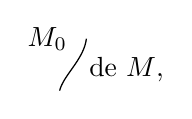
\begin{tikzpicture}[x=1cm,y=1cm]
\node[anchor=base east,inner sep=0] at (0.45,0.38) {\inserted{$M_0$}};
\node[anchor=base west,inner sep=0] at (0.72,0) {de $M$,};
\draw[line width=0.45pt] (0.69,0.48) .. controls (0.66,0.22) and (0.40,0.02) .. (0.35,-0.18);
\end{tikzpicture}%
}
où \deleted{\unsure{de}} $\mathcal F_0$ de $M$. \deleted{On \unsure{définit}} \deleted{L'application \unsure{du|de} cosupport \unsure{d|de}} On \unsure{désidentifie|identifie} $\Sigma$ de \deleted{$\unsure{\mathscr P|\mathcal F}$} ses deux
% R2-realisations-points: two detached low points, with no assigned punctuation function.
\figure{%
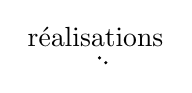
\begin{tikzpicture}[x=1cm,y=1cm]
\node[anchor=base west,inner sep=0] at (0,0) {\unsure{réalisations}};
\fill (0.92,-0.14) circle[radius=0.022cm];
\fill (1.00,-0.20) circle[radius=0.022cm];
\end{tikzpicture}%
}
(comme \unsure{partie|parties} de $\unsure{\mathscr P|\mathcal P|\wp|P}(M)$, ou de $\mathscr P(\mathcal F)$) et on écrit, pour $\sigma\in\Sigma$
\[
M_\sigma\subset M,\qquad\mathcal F_\sigma\subset\mathcal F
\]

Dans $\Sigma$, \deleted{pour} la notion de cosupport est une
% R2-anti-overwrite: one crowded correction area; the old and final layers are not successive words.
\figure{%
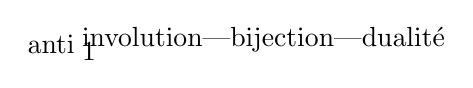
\begin{tikzpicture}[x=1cm,y=1cm]
\node[anchor=base west,inner sep=0] at (0,0) {anti};
\node[anchor=base west,inner sep=0] at (0.69,-0.08) {\deleted{\illegible{1}}};
\node[anchor=base west,inner sep=0] at (0.69,0.09) {\unsure{involution|bijection|dualité}};
\end{tikzpicture}%
}
d'ens. ordonnés. Dans $\Sigma$, on a des $\mathrm{Inf}$ quelconques (c'est l'intersection des parties de $M$, ou de $\mathcal F$), et des $\mathrm{Sup}$ quelconques (c'est la partie saturée
